\documentclass[11pt]{article}

\usepackage{amsmath}
\usepackage{booktabs}
\usepackage{graphicx}
\usepackage{epstopdf}
\usepackage{hyperref}
\usepackage{url}
\usepackage[margin=1in]{geometry}

\title{Do Selected Neural and Zero-Shot Time-Series Models Beat Persistence in Absolute Stock-Price Forecasting? A Cross-Market Audit}

\author{Chu-Nuo Tan\\

Guangzhou Maritime University\\
Guangzhou, China}

\date{}

\begin{document}
\maketitle

\begin{abstract}
Supervised neural and zero-shot time-series forecasting models are increasingly applied to financial price prediction, but many stock-price studies still evaluate models before verifying whether they outperform a no-training persistence rule. This paper presents a cross-market baseline-first audit of absolute stock-price level forecasting. The study evaluates 165 dataset-series memberships, corresponding to 133 unique ticker symbols after cross-index overlaps, from U.S., Hong Kong, and global ETF universes over 2015 to 2026, two price modes, three horizons, and matched chronological train/validation/test splits. The audited models include LSTM, GRU, DLinear, scaled-down PatchTST-style, iTransformer-style, and TimeMixer-style supervised implementations, plus Chronos-T5-small zero-shot forecasting. Other foundation models are discussed but not experimentally evaluated. The primary usefulness gate is latest-close persistence on the same test origins. Across 35,640 supervised neural configuration-seed rows, only 23 beat latest-close persistence. Chronos-T5-small has 133 passes among 990 sampled-origin rows, but direct pass-count comparison is protocol-confounded and its median RMSE ratio remains above persistence at 1.035. The evidence supports a negative but bounded conclusion: for absolute stock-price level regression, compact learned forecasters and one small foundation model should be treated with caution and should not be claimed useful without first clearing a persistence gate. The paper contributes a reproducible baseline-first audit protocol and shows how positive model-comparison claims can disappear once persistence is treated as the primary benchmark rather than an afterthought.
\end{abstract}

\noindent\textbf{Keywords:} stock forecasting; persistence baseline; time-series foundation models; Chronos; PatchTST; iTransformer; TimeMixer; negative results

\section{Introduction}

Stock-price forecasting remains a common applied machine-learning problem. A typical study gathers daily OHLCV data, adds technical indicators, trains a neural network, and reports RMSE, MAE, or MAPE on a held-out period. More recent versions of this workflow replace recurrent networks with transformer-based or foundation-style time-series models. However, a central evaluation problem remains: absolute stock prices are highly persistent. If the target is the future price level, the no-training rule that the future close equals the latest observed close is often extremely hard to beat.

This observation changes the order of evidence required for a credible paper. Before asking whether one architecture is better than another, the first question is whether any learned model adds value beyond latest-close persistence on the same chronological test labels. If the answer is no, then claims about feature engineering, architectural novelty, or model sophistication are not supported for this target.

The original version of this project was a conventional applied stock-prediction study using LSTM/GRU models and technical indicators. Expanded audit experiments invalidated that positive framing. The current paper therefore reframes the work as a baseline-first diagnostic audit:

\begin{quote}
Do selected supervised and zero-shot time-series models reliably beat latest-close persistence in absolute stock-price level forecasting?
\end{quote}

Under the audited protocol, the answer is largely negative. Supervised neural models almost never clear the persistence gate. Chronos-T5-small zero-shot forecasting produces more local wins, especially at longer horizons, but remains slightly worse than persistence in median RMSE ratio. This is a stronger and more honest contribution than claiming a fragile positive result from a narrow model comparison.

The paper makes three contributions:
\begin{itemize}
\item It defines a cross-market baseline-first protocol for absolute stock-price forecasting, using matched chronological evaluation and a mandatory persistence gate.
\item It audits recurrent, linear, transformer-style, multiscale, and zero-shot foundation-model forecasters across 165 dataset-series memberships, two price modes, and three horizons.
\item It reports a negative result that is useful for applied researchers: architecture comparisons should be interpreted only after a model beats no-training persistence.
\end{itemize}

\section{Related Work}

\subsection{Financial Time-Series Forecasting}

Neural networks and technical indicators have long been used in financial prediction studies. LSTM-based and hybrid deep-learning pipelines are common because they can process sliding windows and nonlinear features \cite{bao2017deep,patel2015trend}. Recent financial deep-learning surveys show the breadth of applications and the continuing difficulty of reliable financial prediction \cite{sezer2020stockreview,ozbayoglu2020financialsurvey}. These studies often emphasize relative performance among learned models. For absolute price-level prediction, however, persistence is not a weak baseline; it is the natural first-order comparator. This baseline-first stance is consistent with the broader finance literature on unstable out-of-sample predictability, where simple historical or persistence-like benchmarks are difficult to improve upon \cite{campbell2008predicting,welch2008comprehensive}.

\subsection{Modern Time-Series Models}

Recent forecasting research has produced architectures that patch, invert, decompose, or mix temporal representations. Deep forecasting surveys summarize the rapid architectural diversification of this area \cite{lim2021survey,benidis2022tutorial}. DLinear challenged the value of large transformer models for long-horizon forecasting \cite{zeng2023transformers}. PatchTST applies patch-based transformer modeling to multivariate time series \cite{nie2023patchtst}. iTransformer inverts the usual tokenization scheme and treats variates as tokens \cite{liu2024itransformer}. TimeMixer uses multiscale mixing to combine decomposed temporal patterns \cite{wang2024timemixer}. These models are relevant because they represent current forecasting practice beyond recurrent networks.

\subsection{Foundation Models for Forecasting}

Chronos casts time-series forecasting as a language-model-like sequence modeling problem over quantized values \cite{ansari2024chronos}. It is part of a broader foundation-model trend that includes decoder-only and general-purpose time-series models such as Lag-Llama, TimesFM, MOMENT, and Moirai \cite{rasul2023lagllama,das2024timesfm,goswami2024moment,woo2024moirai}. Such zero-shot forecasters are attractive for applied finance because they avoid per-asset training. Yet zero-shot convenience does not remove the need for a persistence gate. A foundation model that is broadly competent may still underperform the latest observed close for price-level stock forecasting.

\section{Audit Protocol}

\subsection{Data}

The audit uses daily Yahoo Finance data from 2015-01-02 to 2026-04-30 after download cleaning. The cross-market universe contains 165 successful dataset-series memberships across five configured lists: Dow 30, Nasdaq large-technology stocks, an S\&P 100 subset, Hang Seng large-cap stocks, and a global ETF basket. Because some U.S. tickers appear in more than one configured list, these memberships correspond to 133 unique ticker symbols after cross-index overlaps. One configured Hong Kong ticker failed download and is excluded from the analyzed universe.

Two price modes are evaluated. The raw-close mode uses the downloaded OHLCV fields directly. The adjusted-close mode adjusts OHLC prices by the adjusted-close to close ratio, preserving the same volume field. Horizons are 1, 5, and 10 trading days. The target is the future absolute closing price level, not return, direction, volatility, or trading profit.

\input{tables/crossmarket_core_tables}

\subsection{Splitting and Baselines}

Each asset is split chronologically into 72\% training, 8\% validation, and 20\% testing. Feature scalers are fit only on the training segment and then applied to validation and test segments. Hyperparameter and checkpoint selection use validation loss only. Test labels are never shuffled.

The primary gate is latest-close persistence: at each test origin, the forecast equals the close at that origin. Additional no-training baselines, including drift-adjusted persistence and rolling means, are computed as diagnostics, but latest-close persistence is the mandatory minimum usefulness gate because it is simple, transparent, and matched to the absolute-price target.

For assets with the full downloaded calendar, the nominal data span is 2015-01-02 to 2026-04-30, with the chronological split falling approximately in early 2023 for the train/validation boundary and late 2023 for the validation/test boundary. Exact split rows vary slightly by market calendar and indicator availability and are stored in the evidence package. The adjusted-close mode multiplies same-day OHLC prices by the same-day adjusted-close to close ratio; it does not use future adjustment information beyond what is present in the downloaded daily record.

\subsection{Models and Implementation Scope}

The supervised audit includes LSTM, GRU, DLinear, scaled-down PatchTST-style, scaled-down iTransformer-style, and scaled-down TimeMixer-style implementations. The word ``style'' is important: these are compact audit implementations, not official full-capacity reproductions of the published architectures. They are included to stress-test the baseline-first claim across several architectural motifs, not to rank official model repositories. Therefore, the results should not be interpreted as a definitive performance assessment of the full PatchTST, iTransformer, or TimeMixer systems.

All supervised models use a direct forecasting setup: for each horizon, a separate target is constructed by shifting the close price by that horizon, rather than iterating a one-step model. The main cross-market runs use a 60-trading-day input window, hidden dimension 64, dropout 0.1 where applicable, AdamW with learning rate 0.001, early stopping on validation loss, and seeds 42, 123, and 777. LSTM and GRU use one recurrent layer. DLinear applies a linear temporal projection followed by a feature head. The PatchTST-style proxy uses patch length 10, stride 5, two transformer encoder layers, four attention heads, GELU activation, and feed-forward dimension four times the model dimension. The iTransformer-style proxy treats variables as tokens, embeds each variable's full temporal trace, and uses two transformer encoder layers with four heads. The TimeMixer-style proxy concatenates representations at scales 1, 2, and 4 and passes them through a two-layer GELU MLP.

Each supervised model is evaluated over all assets, two price modes, three horizons, two feature sets, and three random seeds, yielding 5,940 rows per supervised model. The feature sets are OHLCV and OHLCV plus RSI, MACD, and Bollinger-band indicators.

The zero-shot audit uses Chronos-T5-small with univariate close-price contexts of up to 512 observations and 20 generated samples per forecast. Because zero-shot generation is more expensive and does not have the same training loop as the supervised models, it is evaluated using a sparse sampled-origin protocol: up to 96 test origins are selected by evenly spacing indices across each test segment for each asset-price-horizon combination. This creates 990 Chronos rows. Chronos results are therefore reported separately as a foundation-model audit rather than merged as if they were identical to the supervised full rolling-origin protocol. With a full rolling-origin evaluation, Chronos pass rates and tail behavior could shift.

\subsection{Metrics and Statistical Tests}

For each row, the audit records RMSE, MAE, MAPE, and the ratio between model RMSE and latest-close RMSE. Ratios below 1.0 pass the persistence gate; ratios above 1.0 fail it. Model-level summaries report pass count, pass rate, median RMSE ratio, and bootstrap 95\% confidence intervals for the median. A one-sided Wilcoxon signed-rank test evaluates whether model RMSE ratios are greater than 1.0. Because rows share tickers, horizons, price modes, seeds, and model families, the inferential summaries are interpreted as paired diagnostic evidence under this audit design rather than as independent-sample claims over unrelated observations.

\section{Results}

\begin{figure}[t]
\centering
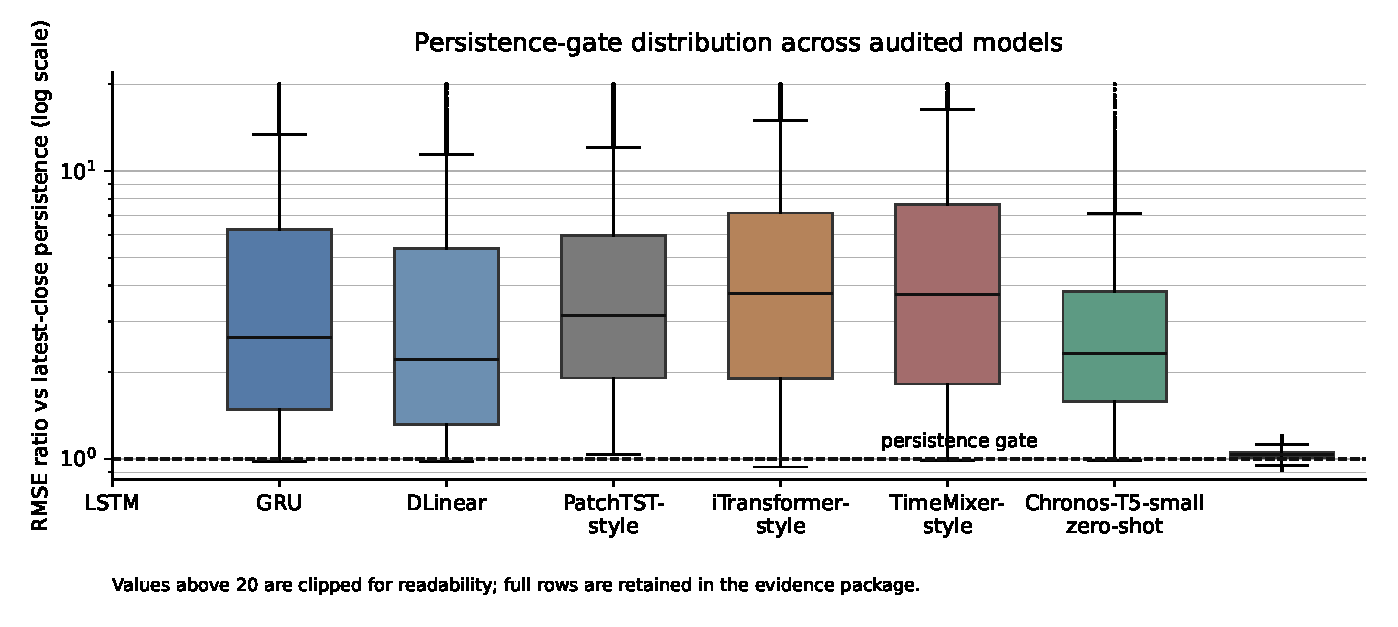
\includegraphics[width=0.92\textwidth]{figures/Figure1_RMSE_Ratio_Distribution.eps}
\caption{Distribution of RMSE ratios relative to latest-close persistence. Values below the dashed line beat persistence; values above it underperform. The supervised compact implementations are evaluated with full rolling-origin tests, while Chronos-T5-small uses the sampled-origin zero-shot protocol. Extreme ratios above 20 are clipped only for visualization.}
\label{fig:rmse_ratio_distribution}
\end{figure}

\subsection{Supervised Models Rarely Pass}

Table~\ref{tab:model_gate_summary} and Fig.~\ref{fig:rmse_ratio_distribution} show the central result. Across 35,640 supervised neural rows, only 23 pass the persistence gate. LSTM passes 8 of 5,940 rows, GRU passes 5, DLinear passes none, and the three scaled-down modern implementations pass only 10 rows combined. The median RMSE ratios are all far above 1.0, ranging from 2.221 for GRU to 3.766 for PatchTST-style. These are not small losses to persistence; they are systematic underperformance relative to a no-training baseline under this absolute-price protocol.

The horizon breakdown in Table~\ref{tab:horizon_summary} shows that longer horizons are somewhat easier, but the conclusion does not change. All supervised model groups have median RMSE ratios above 1.0 at 1-day, 5-day, and 10-day horizons. The 1-day case is especially severe because latest-close persistence is nearly aligned with the target.

\subsection{Chronos Has Local Wins But Not a Stable Advantage}

Chronos-T5-small is meaningfully different from the supervised models. It passes 133 of 990 sampled-origin rows. The nominal pass rate of 13.4\% exceeds that of the supervised models, but direct row-count comparisons are confounded because Chronos was evaluated on a sparse sampled-origin protocol rather than the full rolling-origin protocol used for the supervised models. Therefore, the more reliable aggregate statistic is the median RMSE ratio, which remains above 1.0. Its best cases include individual ETFs, U.S. stocks, and Hang Seng stocks where RMSE ratios fall below 0.95. This suggests that zero-shot foundation forecasters can sometimes improve on latest-close persistence.

However, the aggregate result remains negative. Chronos has median RMSE ratio 1.035 with a bootstrap 95\% confidence interval of [1.033, 1.037]. The one-sided Wilcoxon test strongly rejects equality in the direction of ratios above 1.0. Because the sampled origins may yield less stable tail estimates, the observed pass count should be interpreted as evidence that zero-shot forecasting can occasionally surpass persistence, not as evidence that Chronos-T5-small consistently outperforms the latest close. To verify that sparse origin sampling does not drive this interpretation, we also ran a full-origin Chronos subset covering two assets per dataset, both price modes, and all three horizons. In that 60-row verification, Chronos passed only 2 rows and had a median RMSE ratio of 1.028, consistent with the main sampled-origin conclusion.

\subsection{Cross-Market Pattern}

The underperformance is not confined to a single asset list. Supervised models fail to clear the persistence gate across U.S. large-cap equities, technology-heavy equities, Hong Kong large caps, and ETFs. Hang Seng assets produce more of the rare supervised passes, and ETFs produce the highest Chronos pass rate, but no dataset reverses the overall conclusion. The audit therefore supports a bounded cross-market claim: for price-level forecasting, compact learned forecasters and Chronos-T5-small do not automatically translate model sophistication into out-of-sample improvement over latest-close persistence.

\section{Discussion}

\subsection{Why Persistence Is Hard to Beat}

Absolute price levels contain a strong identity component: the next close is usually close to the current close. A learned model trained with sliding windows must estimate both the level and the small future change. Even when it learns the broad level, small lag or smoothing errors can dominate the RMSE difference against persistence. This explains why visually plausible neural predictions can still fail the gate.

\subsection{What the Negative Result Means}

The result does not show that financial forecasting is impossible. It also does not evaluate return prediction, direction classification, volatility forecasting, ranking, portfolio construction, or trading profitability. The conclusion is narrower and more useful: for absolute stock-price level regression, no-training persistence must be passed before claims about architecture, indicators, or foundation models are credible.

\subsection{Implications for Applied Papers}

Applied stock-prediction papers should report persistence baselines as primary evidence, not as a supplementary sanity check. If a model fails persistence, comparisons among learned models should be presented as engineering diagnostics rather than forecasting usefulness. If a model passes persistence only in selected assets or horizons, the claim should be local and conditional rather than general.

Even these compact implementations capture core architectural motifs that distinguish modern forecasters, including patching, channel-wise attention, and multiscale mixing. Their underperformance reinforces the baseline-first message, although official full-scale reproductions would still be required for model-specific conclusions about the published architectures.

\section{Limitations}

First, the compact PatchTST-style, iTransformer-style, and TimeMixer-style implementations are audit implementations rather than full official reproductions. They are useful for broad stress testing, but official implementations and larger hyperparameter sweeps would be needed for model-specific claims. Second, the Chronos experiment uses Chronos-T5-small and sampled origins. Larger foundation models, including TimesFM, Lag-Llama, MOMENT, Moirai, or larger Chronos variants, may behave differently. Third, the target is absolute price level. Other financial targets require different baselines and should not be inferred from this audit.

\section{Reproducibility Materials}

The project stores the audit protocol, figure-generation script, raw download summaries, model-level CSV files, and generated evidence tables with the manuscript. The main evidence package contains the combined model-result table, dataset coverage table, model-gate summary, horizon summary, dataset-model summary, best and worst row extracts, and the LaTeX table source used in this paper. This organization is intentional: the main manuscript reports only the compact evidence needed to evaluate the claim, while the CSV artifacts preserve ticker-level, seed-level, feature-set, horizon, and protocol-level details for independent inspection.

The most important reproducibility rule is that the persistence gate is computed on the same chronological labels as each model result. This avoids a common evaluation error in which a neural model is compared against a baseline using a different test window, different normalization, or different label alignment. The code therefore treats the baseline as part of the experimental protocol rather than as a post-hoc descriptive statistic.

\section{Data and Code Availability}

The raw input data are daily OHLCV files downloaded from Yahoo Finance for the audited tickers. The Python scripts used for data auditing, model evaluation, figure generation, evidence-table generation, and PDF compilation are available together with processed CSV result files and the supplementary evidence package in a public GitHub repository archived on Zenodo: \url{https://doi.org/10.5281/zenodo.20412777}. The supplement reports the nominal chronological split boundaries, and the full model-result CSV files record row-level train, validation, and test sample counts.

\section{Conclusion}

This paper audits whether compact modern time-series forecasters and Chronos-T5-small beat latest-close persistence in cross-market stock-price level prediction. The answer is mostly no under the audited protocol. Supervised neural models almost never pass the persistence gate, and Chronos-T5-small zero-shot forecasting, while locally competitive, remains slightly worse than persistence in median RMSE ratio. The main contribution is therefore methodological: baseline-first evaluation prevents weak positive claims from surviving merely because a learned model looks sophisticated or beats another learned model. For absolute stock-price forecasting, persistence is not optional background; it is the first gate.

\begin{thebibliography}{99}

\bibitem{bao2017deep}
W. Bao, J. Yue, and Y. Rao, ``A deep learning framework for financial time series using stacked autoencoders and long-short term memory,'' \emph{PLOS ONE}, vol. 12, no. 7, 2017.

\bibitem{patel2015trend}
J. Patel, S. Shah, P. Thakkar, and K. Kotecha, ``Predicting stock and stock price index movement using trend deterministic data preparation and machine learning techniques,'' \emph{Expert Systems with Applications}, vol. 42, no. 1, pp. 259--268, 2015.

\bibitem{sezer2020stockreview}
O. B. Sezer, M. U. Gudelek, and A. M. Ozbayoglu, ``Financial time series forecasting with deep learning: A systematic literature review: 2005--2019,'' \emph{Applied Soft Computing}, vol. 90, 2020.

\bibitem{ozbayoglu2020financialsurvey}
A. M. Ozbayoglu, M. U. Gudelek, and O. B. Sezer, ``Deep learning for financial applications: A survey,'' \emph{Applied Soft Computing}, vol. 93, 2020.

\bibitem{campbell2008predicting}
J. Y. Campbell and S. B. Thompson, ``Predicting excess stock returns out of sample: Can anything beat the historical average?'' \emph{Review of Financial Studies}, vol. 21, no. 4, pp. 1509--1531, 2008.

\bibitem{welch2008comprehensive}
I. Welch and A. Goyal, ``A comprehensive look at the empirical performance of equity premium prediction,'' \emph{Review of Financial Studies}, vol. 21, no. 4, pp. 1455--1508, 2008.

\bibitem{hyndman2018forecasting}
R. J. Hyndman and G. Athanasopoulos, \emph{Forecasting: Principles and Practice}, 2nd ed. OTexts, 2018.

\bibitem{makridakis2018concerns}
S. Makridakis, E. Spiliotis, and V. Assimakopoulos, ``Statistical and machine learning forecasting methods: Concerns and ways forward,'' \emph{PLOS ONE}, vol. 13, no. 3, 2018.

\bibitem{lim2021survey}
B. Lim and S. Zohren, ``Time-series forecasting with deep learning: A survey,'' \emph{Philosophical Transactions of the Royal Society A}, vol. 379, no. 2194, 2021.

\bibitem{benidis2022tutorial}
K. Benidis et al., ``Deep learning for time series forecasting: Tutorial and literature survey,'' \emph{ACM Computing Surveys}, vol. 55, no. 6, 2022.

\bibitem{zeng2023transformers}
A. Zeng, M. Chen, L. Zhang, and Q. Xu, ``Are transformers effective for time series forecasting?'' in \emph{Proceedings of the AAAI Conference on Artificial Intelligence}, 2023.

\bibitem{nie2023patchtst}
Y. Nie, N. H. Nguyen, P. Sinthong, and J. Kalagnanam, ``A time series is worth 64 words: Long-term forecasting with transformers,'' in \emph{International Conference on Learning Representations}, 2023.

\bibitem{liu2024itransformer}
Y. Liu, T. Hu, H. Zhang, H. Wu, S. Wang, L. Ma, and M. Long, ``iTransformer: Inverted transformers are effective for time series forecasting,'' in \emph{International Conference on Learning Representations}, 2024.

\bibitem{wang2024timemixer}
S. Wang, H. Wu, X. Shi, T. Hu, H. Luo, L. Ma, J. Y. Zhang, and J. Zhou, ``TimeMixer: Decomposable multiscale mixing for time series forecasting,'' in \emph{International Conference on Learning Representations}, 2024.

\bibitem{ansari2024chronos}
A. F. Ansari et al., ``Chronos: Learning the language of time series,'' \emph{Transactions on Machine Learning Research}, 2024.

\bibitem{rasul2023lagllama}
K. Rasul et al., ``Lag-Llama: Towards foundation models for probabilistic time series forecasting,'' \emph{arXiv preprint arXiv:2310.08278}, 2023.

\bibitem{das2024timesfm}
A. Das et al., ``A decoder-only foundation model for time-series forecasting,'' in \emph{Proceedings of the International Conference on Machine Learning}, 2024.

\bibitem{goswami2024moment}
M. Goswami et al., ``MOMENT: A family of open time-series foundation models,'' in \emph{Proceedings of the International Conference on Machine Learning}, 2024.

\bibitem{woo2024moirai}
G. Woo et al., ``Unified training of universal time series forecasting transformers,'' in \emph{Proceedings of the International Conference on Machine Learning}, 2024.

\end{thebibliography}


\end{document}
